\documentclass[a4paper]{article}

\usepackage[english]{babel} \usepackage{hyperref} \usepackage{float}
\usepackage[utf8]{inputenc} \usepackage{amsmath} \usepackage{graphicx}
\usepackage[colorinlistoftodos]{todonotes} \usepackage{tikz}
\usepackage{pdfpages} \usepackage{listings}
\usepackage{listings}
\usepackage{color}

\definecolor{green}{rgb}{0,0.6,0}
\definecolor{gray}{rgb}{0.5,0.5,0.5}
\definecolor{mauve}{rgb}{0.58,0,0.82}

\lstset{frame=tb,
  language=Java,
  aboveskip=3mm,
  belowskip=3mm,
  showstringspaces=false,
  columns=flexible,
  basicstyle={\small\ttfamily},
  numbers=left,
  numberstyle=\tiny\color{gray},
  keywordstyle=\color{blue},
  commentstyle=\color{green},
  stringstyle=\color{mauve},
  breaklines=true,
  breakatwhitespace=true,
  tabsize=3
}

\lstset{emph={%  
    for%
    },emphstyle={\color{blue}\bfseries}%
}%

\lstset{escapeinside={(*@}{@*)}}

\renewcommand{\lstlistingname}{Algorithm}

\usetikzlibrary{arrows,positioning,shapes.geometric}

\title{Dynamic A* on \emph{GPU}}
\usepackage{listings}
\usepackage{color}


\author{\normalsize Lokesh Koshale (CS15B049) \\\normalsize}

\date{\color{black}August 23 2019}

\begin{document} \maketitle


% \section{Abstract}
%  We propose algorithm and techniques to solve the dynamic A star guided search on GPU.
% The goal of a dynamic graph algorithm is to
% support query and update operations as
% quickly as possible.

% In many applications graphs are subject to discrete changes, such as additions or deletions
% of edges or vertices.

% The goal of
% a dynamic graph algorithm is to update efficiently the solution of a problem after dynamic changes,
% rather than having to recompute it from scratch each time

\section{Introduction}
A*\cite{A*}\cite{Wiki A*} is one of widely used path planning and shortest path approximation algorithm. It is used widespread due to its performance and accuracy. It is used to find shortest path in maps and games where there can be hindrances. In most of real life cases the graph is not static and is constantly changing. D*\cite{original D*}, focused D*\cite{focused D*} and D* lite\cite{D* Lite} are a family of informed incremental search algorithm where edge cost can change while we try to find the optimal path. We solve the problem where edges can be inserted OR deleted from the graph where the number of nodes are fixed. We assume that graph doesn't change while we are finding the optimal path.
\begin{lstlisting}[language=C , caption=A*\cite{A*} ]
Input: A Graph(V,E) with source node (*@\textit{start}@*) and goal node (*@\textit{end}@*).
Output: Least cost path from (*@\textit{start}@*) to (*@\textit{end}@*).
Steps:
Initialize 
    open_list = {(*@\textit{start}@*)}          /* list of nodes to be traversed */
    closed_list = {}              /* list of already traversed node */
    g(start) = 0                  /* cost from source node to node */
    h(start) = heuristic_function(start,end) /* estimated cost from source to goal node */
    f(start) = g(start) + h(start)      /* total cost from goal to node */
    
    while open_list is not empty:
        m = node on top of open_list with least f
        if m == end
            return
        remove m from open_list
        add m to close list
        
        for each n in child(m):
            cost = g(m) + distance(m,n)
            
            if n in open_list and cost < g(n):
                remove n from open_list as new path is better.
                
            if n in closed_list and cost < g(n):
                remove n from closed_list
                
            if n is not in open_list and closed_list:
                g(n) = cost
                h(n) = heuristic_function(n,end)
                f(n) = g(n) + h(n)
                add n to open_list
    
    return failure
    
\end{lstlisting}
General purpose computation on graphics processing units (GPGPU) has been widely used to accelerate numerous computational task. In multicore systems to improve the performance one has to increase the number of cores and adding more and more cores increase the cost thus GPU is rising as cost efficient hardware to execute parallel algorithms with better performances. In paper \textit{Massively Parallel A* Search on a GPU}\cite{GA*} the authors proposed a parallel variant of A* for GPU, we borrow the parallelization of A* on GPU from them. The bottle neck for parallelization is the sequential nature of Priority Queue which is the primary data structure to implement A*, to utilise the numerous cores of GPU the authors proposes to have multiple priority queues thus expanding many nodes at once. In paper author claims that GA* gives 30x-45x performance improvement from the CPU implementation.
\begin{lstlisting}[language=FORTRAN, caption=GA*]
procedure GA*(s,t,k)   !find the shortest path from s to t with k queues
Let (*@$\{Q_i\}^k_{i=1} $@*) be the priority queues of open_list
Let H be the closed list
PUSH((*@$Q_1$@*), s)
m (*@$\leftarrow$@*) nil         !m stores the best target state
while (*@$Q$@*) is not empty do:
    Let (*@$S$@*) be an empty list
    for i (*@$\leftarrow$@*) 1 to k in parallel do:
        if (*@$Q_i$@*) is empty then
            continue
        end if
        (*@$q_i \leftarrow$@*) Extract((*@$Q_i$@*))
        if (*@$q_i.node = t$@*) then:
            if m = nil or (*@$f(q_i) < f(m)$@*) then:
                m (*@$\leftarrow q_i$@*)
            end if
            continue
        end if
        (*@$S \leftarrow S + EXPAND(q_i)$@*)
    end for
    
    if m (*@$\neq$@*) nil and (*@$f(m) \leq min_{q\in Q}f(q)$@*) then:
        return the path generated from m
    end if

    (*@$T \leftarrow S$@*)
    for (*@$s'\in S$@*) in parallel do:
        if (*@$s'.node \in H$ @*) and (*@$H[s'.node].g < s'.g$@*) then:
            remove (*@$s'$@*) from (*@$T$@*)
        end if
    end for
    
    for (*@$t' \in T$@*) in parallel do:
        (*@$t'.f \leftarrow f(t')$@*)
        PUSH (*@$t'$@*) to one of priority queues
        (*@$H[t'.node] \leftarrow t'$@*)
    end for
end while

end procedure
    

\end{lstlisting}
% \section{Properties of A*}
When we complete the A* search we get some useful information about each of the nodes in the graph. Below we make certain claims and prove them, which will be later useful in deriving some major algorithmic choices for processing addition and deletion of edges.\\
\textbf{Lemma 1:}\textit{If we have found a node $d$ which have cost $f_d$ then all the nodes $i \in V$ which have have cost $f_i < f_d$ are already visited(expanded).}\\
\textbf{Proof:} Suppose we found the node $d$ with cost $f_d$ and there exists a node n such that node $n$ is not visited i.e $n \notin closed\_list$ and $f_n < f_d$\\
If $n \notin closed\_list$ then either node $n \in open\_list$ or $n$ is not explored yet which means $f_n = \infty $.\\
If $n \in open\_list$  and we know that $f_n < f_d$, In A* to expand a node we always chose the node with least $f$ ( as in line no 15 of Algorithm 1:A*).So $n$ should be chosen before $d$ and which implies that $n$ is already visited(expanded). which contradicts our assumption that $n$ is not visited.\\
If $f_n = \infty $, we have found the node $d$ so $f_d \neq \infty$ which implies $f_n > f_d$ which violates our assumption that $f_n <  f_d$.\\
hence proved.\\
\textbf{corollary:}\textit{If some nodes are not visited at the end of A* then the actual cost of all those node will be greater than or equal to the cost of destination. }

\section{Incremental}
In Incremental setting there are only edge-insertions, i.e edge $u \rightarrow v $ is added in G where $u\in V $ and $v \in V$.\\
\\
\begin{center}
    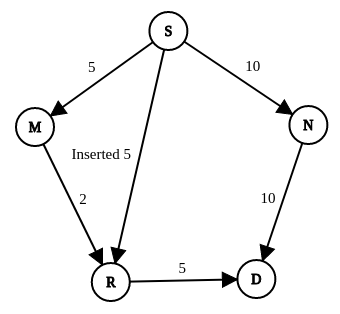
\includegraphics[scale=0.4]{img/insert1.png}
\end{center}
In the above graph the Optimal Path before insertion was $S \rightarrow M \rightarrow R \rightarrow D$, when we insert edge $S \rightarrow D$, the cost $f$ of node $R$ changes and Optimal Path changes to $S \rightarrow R \rightarrow D$.\\

\textbf{Lemma 2:} \textit{Insertion of an edge can not increase the cost of source to destination Optimal Path.}\\
\textbf{Proof:} Suppose we add and an edge $u \rightarrow v $ with weight $w_{uv}$ where $u \in V$ and $v \in V$. The cost of reaching $v$ from source using edge $u \rightarrow v$ is $g(v)_{new} = g(u) + w_{uv}$. There can be two cases:\\
\textit{Case 1:} If $g(v)_{new} < g(v)$, let if optimal path consist of node $v$ then the decrease of cost of $v$ will decrease the cost of Optimal Path. If $v$ doesn't belong to optimal path then, if there is path from $v$ to destination and source $\rightarrow v \rightarrow$ destination cost is less then Optimal then it becomes the new Optimal Path with lesser cost, if it doesn't then the Optimal Path remains same.\\
\textit{Case 2:} If $g(v)_{new} \geq g(v)$,  Suppose node $v$ is our destination, from definition Optimal Path is a path with least cost associated with it, so the optimal cost to reach $v$ is $g(v)$, so the addition of this edge has no affect on cost of any node of graph which implies the cost of Optimal Path remains same.\\
In both cases cost of Optimal Path doesn't increase, Hence Proved\\
\\
\textbf{Lemma 3:} \textit{If we add an edge $u \rightarrow v$ and $f(u) > f(destination)$ then addition of this edge will not affect the Optimal Path.}\\
\textbf{Proof:}Given  $f(destination) < f(u)$, As weights are positive $w_{uv} > 0$ so  cost of any path from source $\rightarrow u \rightarrow v$ will be $g(u) + $ cost of reaching destination from $u$ as $g(u) > g(destination)$ the cost of such paths will always be larger and hence can't be the Optimal Path so the addition of such edges doesn't affect the Optimal Path.\\   
\textbf{corollary:} \textit{If If we add an edge $u \rightarrow v$ and $f(u) = \infty$ then addition of this edge will not affect the optimal path.}\\
\textbf{Proof:} If $f(u) = \infty$ then $f(u) > f(destination)$ so it follows from Lemma 3 that addition of such edges doesn't affect the optimal path.\\
\\
We know from Lemma 1 that insertions can't increase the cost of optimal path but they can decrease the cost, and there can be a new optimal path from the inserted edge. Also if we insert the $u \rightarrow v$ and $g(v)$ changes then all its descendants in the graph whose $g$ are computed based on $v$ are stale values. There can be two approaches to update the cost of graph due to this insertions either \textit{propagate} the new value as insertion took place or compute the new value on demand when necessary i.e \textit{lazy update}. We prefer the first one as it simplifies a lot of computation.\\

\subsection{Batch Insertion}

Instead of adding each edge one by one, we process a group of edges inserted at a particular instance of time to utilise the parallelism and computation power of GPU. First, we make an update\_list of vertices from the inserts as if $u \rightarrow v $ is inserted and $f$ of $v$ changes then we add $v$ to update\_list. Then until update\_list is empty we expand each children of nodes in update\_list and if the cost of child is less we add the child in update\_list.
\begin{lstlisting}[language=python, caption=Propagation of Insertions]
procedure: propagate_insertions( list< pair<u,v> > Inserts, E, N):
    update_list = make_update_list(Inserts);
                          
    while update_list not empty:
        s = size(update_list)
        #array of N elements initialized to 0
        flag = array(N,0)
        #s parallel
        expand(update_list,s,flag)
        #create update list from flag
        update_list = generate_update_list(flag)
        
#GPU kernel
procedure: expand(update_list,s,flag):
    id = global_thread_id;
    node = update_list[id];
    
    for each child ch of node:
        lock(ch)
        if f(ch) > g(node) + weight(node,ch) + h(ch):
            f(ch) = g(node) + weight(node,ch) + h(ch)  
            optimal_parent[ch] = node
            flag[ch] = 1
        unlock(ch)


\end{lstlisting}

At the end of propagation if there is change in optimal path then it would also be propagated we prove the same below.\\
\\
\textbf{Lemma 4:}\textit{At the end of propagation $f(destination)$ is the optimal cost of reaching destination from source in the new graph G(V, E+Inserts ).}\\
\textbf{Proof:}
\\

\section{Decremental}
In Decremental setting there are only removal of edges $u \rightarrow v$ where $u \in V$ and $v \in V$. Below we prove some important properties that holds when we remove edges from graph. The following properties holds when we have the Optimal Path for the graph before deletions.\\
\begin{center}
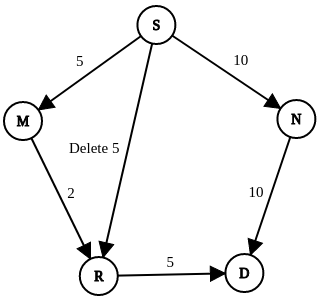
\includegraphics[scale=0.4]{img/Delete2.png}    
\end{center}
In the above graph the Optimal Path before deletion was $S \rightarrow R \rightarrow D$, when we delete the edge $S \rightarrow R$, the Optimal Path changes to $S \rightarrow M \rightarrow R \rightarrow D$.\\
\\
\textbf{Lemma 5:} \textit{Deletion of edge $ u \rightarrow v$ where $u \in V$ and $v \in V$ can not decrease $f(v)$.}
\textbf{Proof:} Let edge$ u \rightarrow v$ get deleted then,\\
\textit{Case 1:} If $u$ is optimal\_parent($v$) then, source $\rightarrow u \rightarrow v$ was optimal the path of reaching $v$ from source, So after deletion, $f_{new}(v) = g(s) + w_{sv} + h(v)$ where $s$ is parent of $v$ with least $g$, In A* we chose the path with least $f$ as we chose $u$ before $s$ implies $f_{new}(v) \geq f_{old}(v)$.\\
\textit{Case 2:} If $u$ is  not the optimal\_parent($v$), then let $s$ be the optimal\_parent($v$), deletion of edge $u \rightarrow v$ doesn't affect the $f(v)$ as the least cost of reaching $v$ is from $s$.\\
From above we can say that deletion of edge $u \rightarrow v$ can only increase $f(v)$. Hence Proved.\\


\textbf{Lemma 6:} \textit{If edge($u,v$) $\notin$ Optimal Path, then deletion of such edges doesn't affect the Optimal Path.}\\
\textbf{Proof:} Suppose we delete edge($u,v$) $\notin$ Optimal Path then, as from \textit{Lemma 5} deletion of such edges can only increase $f(v)$ so if there is a path from source $\rightarrow v \rightarrow$ destination then it's cost will be increased, as Optimal Path is least cost path such paths cannot be an Optimal Path, Hence deletion of such edges doesn't affect the Optimal Path.\\

\textbf{Lemma 7:}\textit{If edge(u,v) is deleted and optimal\_parent(v)$\neq$u, then deletion of such edges doesn't affect the Optimal Path.}\\
\textbf{Proof:} If $u$ is  not the optimal\_parent($v$), then let $s =$ optimal\_parent($v$), deletion of edge $u \rightarrow v$ doesn't affect the $f(v)$ as the least cost of reaching $v$ is from $s$, as there is no change in cost of any nodes so Optimal Path remains same.\\

\subsection{Batch Deletion}
Instead of deleting edges one by one we process deletion in batches, where a batch contains all the deleted edges before an query. From \textit{Lemma 5} we know that deletion of edges can increase the optimal cost, to compute the new optimal cost, we first propagate the change in cost due to deletion of edges to all affected nodes and then we check that due to this propagation are we violating the \textit{Lemma 1} which is a essential property to process the updates that will happen afterwards, if it violates \textit{Lemma 1} then we start A* from where we left before i.e using the open\_list we have computed. At the end we will have the new Optimal Path with the optimal cost for new graph encompassing all the deletions.\\
\\
\textit{Propagation for Deletion:}\\
\textit{1.} For each deleted edge $u \rightarrow v$, if $f(v) \neq \infty$ and optimal\_parent($v$)$=u$ then for such edges we compute the cost of reaching $v$ from its parent's and chose the least one as optimal\_parent($v$) and update $f(v)$, if $v$ doesn't have any parent then $f(v)=\infty$, and we add $v$ to update\_list.\\
\\\textit{2.} For each child of nodes in update\_list, we compute the cost $f$ of child with respect to node and If new cost $f$ is more than $f(child)$ and optimal\_parent(child)  is node
     then,we compute the cost of reaching child from all of its parents and update $f$ to the least cost of the parents and set that parent as optimal\_parent. And we add child to next update\_list.\\
 \\  
\textit{3.} We repeat step 1 and 2 until update\_list is empty.\\
\\
Optimal Cost is least cost of reaching the node but we increase the cost of child at step 2 in above procedure, why we do that is because from \textit{Lemma 5} we know that $f$ might increase due to deletion of edges and we need to propagate the updated higher cost. Also since there is no special ordering of nodes to execute the propagation it may happen that while we propagating for a node its sub-graph might already have been updated so to make sure we have latest value among those we choose the least cost parent and then propagate that cost downwards if applicable.\\ \begin{center}
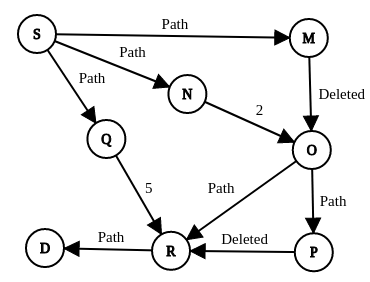
\includegraphics[scale=0.45]{img/Delete1.png}    
\end{center}
In above example the Optimal Path before deletion is $S \rightarrow M \rightarrow O \rightarrow P \rightarrow R \rightarrow D $.
The edges $ M \rightarrow O$ and $P \rightarrow R$ are deleted from graph. So $R,O \in $ update\_list, While propagating for $O$ we might find $R$ again from path $O \rightarrow R$ but $R$ has already updated, if in that update $R$ has chosen path $S \rightarrow M \rightarrow O \rightarrow R$ as its Optimal Path then we have stale value for $f(R)$ as $M \rightarrow O$ is deleted but since $R$'s update happened first it read the stale value before propagation. In such cases we need to find the parent with least cost thus we compute the cost of reaching node from all its parent and choose the parent with least cost as optimal\_parent.

 
\subsection{Deletion and Cycles}
We propagate the deletions so that each node whose cost is already computed will have the latest value. There is a special case of deletions with cycle where even after propagation we can get stale value if we don't perform  certain checks while propagating latest value to nodes. as in given example :

\begin{center}
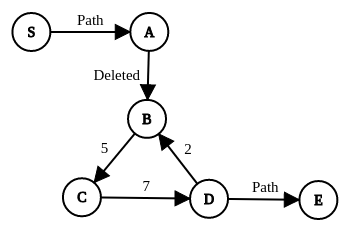
\includegraphics[scale=0.45]{img/cycle.png}        
\end{center}
In The above example the Optimal Path is from $S \rightarrow ABCD \rightarrow E$,where $S$ is source and $E$ is destination. When we remove the edge $A \rightarrow B$, and recompute the $f(B)$, there exist only one parent $D$ so the $f(B)_{new}$ is computed by $f(B)_{new} = g(D) + 2 + h(B)$, which is old value of $g(D)$, as we remove $A \rightarrow B$, there is no path from $S \rightarrow D$ so $g(D)_{new}$ is $\infty$, but we never arrive at that proposition because in propagation of deletion we will propagate from $B$  and $f(D)$ will be updated based on stale value of $f(B)$ and thus we have wrong cost value after deletion of such edges. The main reason this happens is die to the fact that cost $f(D)$ is computed wrt $B$ as $B \in OptimalPath(S,D)$. To avoid such cases, while chosing the optimal\_parent we have to eliminate the parents whose Optimal\_ancestor is current node.\\
\begin{lstlisting}[language=python, caption=Check Cycles]
procedure: check_cycle(node,parent):
    current_node = node
    while there exists optimal_parent(current_node):
        if current_node == parent:
            return true
        current_node = optimal_parent(current_node)
    
    return false
\end{lstlisting}

The propagation for deletion handling all the above cases is given below: 

\begin{lstlisting}[language=python, caption=Propagation of Deletions]
procedure: propagate_deletions( list< pair<u,v> > Deletions, E, N):
     update_list = make_update_list(Deletions);
     
     while update_list not empty:
        s = size(update_list)
        #array of N elements initialized to 0
        flag = array(N,0)
        #s parallel
        expand(update_list,s,flag)
        #create update list from flag
        update_list = generate_update_list(flag)

#GPU kernel
procedure: expand(update_list,s,flag):
    id = global_thread_id;
    node = update_list[id];
    
    for each child ch of node:
        lock(ch)
        if f(ch) < g(node) + weight(node,ch) + h(ch) and optimal_parent[ch] == node:
            
            for all parents p of ch:
                if check_cycle(ch,p) == true:
                    continue
                if f(ch) > g(p) + weight(p,ch) + h(ch):
                    f(ch) = g(p) + weight(p,ch) + h(ch)
                    optimal_parent[ch] = p
            flag[ch] = 1
        unlock(ch)
        
\end{lstlisting}

\textbf{Lemma 8:} \textit{After propagation of deletions if $f(destination) < f(n)$ $ \forall$ $n \in $open\_list then $f(destination)$ is the Optimal Cost of reaching destination from source.}\\
\textbf{Proof:}



%explanation about why we need A* after this.
\section{Fully Dynamic}
Real world graphs are dynamic and edges are changing continuously so there are insertion of edges and deletion of edges at same instance in such cases if a query arrives to find the optima path from source to destination we can retrieve the optimal path without re-executing A* from start again. We have designed the propagation of Insertion( section 4) and propagation of deletions (section 5) such that they can be overlapped and we can process both insertion and deletion at same time by considering them as an update.
\begin{lstlisting}[language=python, caption=Propagation of Updates]
procedure: propagate_updates( list< pair<u,v> > Deletions,list< pair<u,v> > Inserts, E, N):
     update_list = make_update_list_insertion(Inserts);
     update_list = append( update_list, make_update_list_deletion(Deletions) )
     
     while update_list not empty:
        s = size(update_list)
        #array of N elements initialized to 0
        flag = array(N,0)
        #s parallel
        expand(update_list,s,flag)
        #create update list from flag
        update_list = generate_update_list(flag)

#GPU kernel
procedure: expand(update_list,s,flag):
    id = global_thread_id;
    node = update_list[id];
    
    for each child ch of node:
        lock(ch)
        if f(ch) > g(node) + weight(node,ch) + h(ch):
            f(ch) = g(node) + weight(node,ch) + h(ch)  
            optimal_parent[ch] = node
            flag[ch] = 1
        elif f(ch) < g(node) + weight(node,ch) + h(ch) and optimal_parent[ch] == node:
            
            for all parents p of ch:
                if check_cycle(ch,p) == true:
                    continue
                if f(ch) > g(p) + weight(p,ch) + h(ch):
                    f(ch) = g(p) + weight(p,ch) + h(ch)
                    optimal_parent[ch] = p
            flag[ch] = 1
        unlock(ch)
\end{lstlisting}

\textbf{Lemma 9:} \textit{After propagation of updates if $f(destination) < f(n)$ $ \forall$ $n \in $open\_list then $f(destination)$ is the Optimal Cost of reaching destination from source.}

\section{Experimental Results}
%results

\section{Related Work}
%write about D* D* lite
In our case the change in cost of edge can be emulated by deleting that edge and inserting the same with new cost.

\section{Conclusion}




\begin{thebibliography}{} 
    \bibitem{A*} Hart, P.; Nilsson, N.; Raphael, B. (1968), "A Formal Basis for the Heuristic Determination of Minimum Cost Paths", IEEE Trans. Syst. Science and Cybernetics
    \bibitem{original D*}Stentz, Anthony (1994), "Optimal and Efficient Path Planning for Partially-Known Environments", Proceedings of the International Conference on Robotics and Automation
    \bibitem{focused D*}Stentz, Anthony (1995), "The Focussed D* Algorithm for Real-Time Replanning", Proceedings of the International Joint Conference on Artificial Intelligence
    \bibitem{D* Lite}Koenig, S.; Likhachev, M. (2005), "Fast Replanning for Navigation in Unknown Terrain", Transactions on Robotics
    \bibitem{LPA*}Koenig, S.; Likhachev, M.; Furcy, D. (2004), "Lifelong Planning A*", Artificial Intelligence.
    \bibitem{GA*}Yichao Zhou and Jianyang Zeng (2015): Massively Parallel A* Search on a GPU, Twenty-Ninth AAAI Conference on Artificial Intelligence.
    \bibitem{Diff CSR}Gaurav Malhotra, Hitish Chappidi, Rupesh Nasre(2016): Fast Dynamic Graph Algorithms.
    \bibitem{Giuseppe}Giuseppe F. Italiano: Dynamic Graph Algorithms.
    \bibitem{Wiki A*}\texttt{https://en.wikipedia.org/wiki/A*\_search\_algorithm}
    \bibitem{Wiki D*}\texttt{https://en.wikipedia.org/wiki/D*}
        

\end{thebibliography}


% All reduce Graphs
\newpage 
    \section{Appendix} 

% Lockin implementation, K PQ implemetation, GA* implementation, 

\begin{lstlisting}
code
\end{lstlisting}

\end{document}